\section{Decomposition of Multivariate Information}
\subsection{The Structure of Multivariate Information}
Suppose there is a random variable $S$ whose information is provided by a random  $\mathbf{R}=\left({R}_1,{R}_2,\ldots,{R}_{n-1}\right)$, then we try to decompose the information into some information contributed by the subsets of $\mathbf{R}$ individually or jointly.

Consider the case where $\mathbf{R}=\left({R}_1,{R}_2\right)$. The total information ${R_1}$ and ${R_2}$ provided is the mutual
information  $I\left(S;{R}_1,{R}_2\right)$, and their contributions can be divided into three parts. First, the unique information, which means the information only provided by ${R_1}$, or vice versa. Second, the redundancy, which means the same or overlapping information that ${R_1}$ and ${R_2}$ provide. Third, the synergy, which means the information that is provided by the combination of ${R_1}$ and ${R_2}$ while not available from either alone.

Therefore, as is shown in Figure \ref{figl}, the total information can be decomposed into three parts: the synergistic information contributed jointly by ${R_1}$ and ${R_2}$,  the unique information from ${R_1}$ or ${R_2}$, and the redundant information shared by ${R_1}$ and ${R_2}$. So we can identify them as the basic atoms of multivariate information.


 
\begin{figure}[ht]
 
\centering
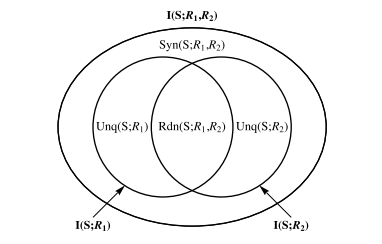
\includegraphics[scale=0.6]{tex/structure3.png}
\caption{Structure of multivariate information for 3 variables}
\label{figl}
 
\end{figure}



Actually, the unique information can be considered as a deformation of synergy or redundancy, so we can say that the multivariate information constitutes of redundancy and synergy.



% 引入我们讨论的信息量
% 给出关键性质


\subsection{Redundancy Measure}

To formally measure the redundancy between multiple collections of sources, we now introduce a redundancy measure $I_{\min}$. Let $A_1, A_2, \ldots, A_k$ be nonempty and potentially overlapping subsets of $\mathbf{R},$ which we call sources. We introduce $I_{\min}$ to measure the information that all sources provide about $S$.

While the specific information $I(S=s ; \mathbf{A})$ quantifies the information associated with a particular outcome of $S$, $I_{\min}$ describes all sources offer to S, or we say "redundancy". Various definitions of specific information have been proposed to quantify different relationships between $S$ and $\mathbf{A}$ but for our purposes the most useful is
\begin{equation}
I(S=s ; \mathbf{A})=\sum_{\mathbf{a}} p(\mathbf{a} | s)\left[\log\frac{1}{p(s)}-\log\frac{1}{p(s |\mathbf{a})}\right]
\end{equation}

To better introduce the meaning of this definition, we use $\frac{1}{p(s)}$ instead of ${p(s)}$. And the former one is called the surprise of $s,$ so $I(S=s ; \mathbf{A})$ is the average reduction in surprise of $s$ given knowledge of $\mathbf{A} .$ In other words, $I(S=s ;\mathbf{ A}$ quantifies the information that $\mathbf{A}$ provides about each particular outcome $s \in S,$ while $I(S ; \mathbf{A})$ is the expected value of this quantity over all outcomes of $S$. Given these considerations, a natural measure of redundancy is the expected value of the minimum information that any source provides about each outcome of $S$.
\begin{definition}[Redundancy Measure]
\begin{equation}I_{\min }\left(S ;\left\{\mathbf{A}_{1}, \mathbf{A}_{2}, \ldots, \mathbf{A}_{k}\right\}\right)=\sum_{s} p(s) \min _{\mathbf{A}_{i}} I\left(S=s ; \mathbf{A}_{i}\right)\end{equation}
where the domain of $I_{\min}$ $\mathcal{A}(\mathbf{R})=\left\{\alpha \in \mathcal{P}_{1}\left(\mathcal{P}_{1}(\mathbf{R})\right): \forall \mathbf{A}_{i}, \mathbf{A}_{j} \in \alpha, \mathbf{A}_{i} \notin \mathbf{A}_{j}\right\}$
\end{definition}
$I_{\min }$ captures the idea that redundancy is the information common to all sources (the minimum information that any source provides $),$ while taking into account that sources may provide information about different outcomes of $S$. Note that, like the mutual information, $I_{\min }$ is also an expected value of specific information terms. And similarly to $I$, $I_{\min }$ also has several useful properties that can be easily proved from its definition.
\begin{itemize}
    \item $I_{\min}$ is non-negative
    \item $I_{\min }$ is less than or equal to $I\left(S ; \mathbf{A}_{i}\right)$ for all $\mathbf{A}_{i}$ 's
    \item For a given source A, the amount of information redundant with $\mathbf{A}$ is maximal for $I_{\min }(S ;\{\mathbf{A}\})=I(S ; \mathbf{A}) .$
\end{itemize}

These properties can confirm $I_{\min}$ with its interpretation as a measure of redundancy.





\subsection{Partial Information Decomposition}
\label{sec:partialdecompositon}

Note that $I_{\min}$ can measure redundancy between collections of sources like $\left\{\left\{R_{1}\right\},\left\{R_{2}, R_{3}\right\}\right\}$ denoted as $\{1\}\{23\}$. A natural observation is that, for any source sets in one collection, if its subsets can always be found at another collection, then it must measure a greater redundancy over the other collection. Therefore, we can define a partial order over the elements of $A(R)$ such that one is considered to precede another if and only if the latter provides any redundant information that the former provides. Formally,
    \begin{equation}\forall \alpha, \beta \in \mathcal{A}(\mathbf{R}), \alpha \preccurlyeq \beta \Leftrightarrow \forall \mathbf{B} \in \beta, \exists \mathbf{A} \in \alpha, \mathbf{A} \subseteq \mathbf{B}\label{partialorder}\end{equation}

And from this partial order, a lattice can be illustrated as follow, which gives us a clear picture of the partial order among collections of sources.(shown in Figure \ref{fig:lattice})



\begin{figure}
            \centering
            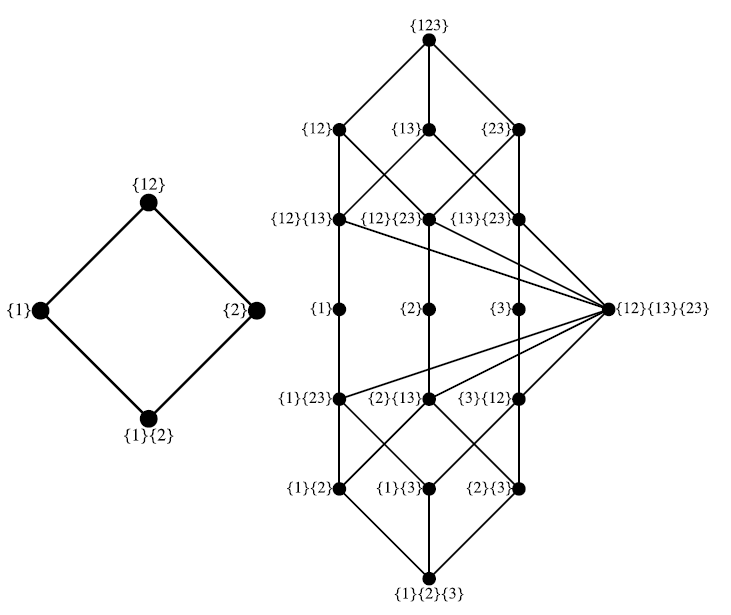
\includegraphics[width=0.6\linewidth]{img/lattic.png}
            \caption{Redundancy lattice for (A) 3 and (B) 4 variables.}
            \label{fig:lattice}
        \end{figure}

The redundant information associated with each node of the redundancy lattice includes, but is not limited to, the redundant information provided by all nodes lower in the lattice. Thus moving from node to node up the lattice, $I_{\min }$ can be thought of as a kind of "cumulative information function," effectively integrating the information provided by increasingly inclusive collections of sources.

The observation above implies that the nodes in the lattice actually would decompose redundancy measure into several non-intersecting fragments and derive an inverse of ${I}_{min}$ called the \textit{partial information function} (PI-function). Whereas ${I}_{min}$ quantifies cumulative information, the PI-function measures the partial information contributed uniquely by each particular collection of sources. This partial information will form the atoms into which we decompose the total information
that $\mathbf{R}$ provides about S. Formally, we define these components with the partial order defined in Equation  \ref{partialorder}.

\begin{definition}[Partial Information]For a collection of sources $\alpha \in \mathcal{A}(\mathbf{R}),$ the PI-function, denoted $\Pi_{\mathrm{R}},$ is defined implicitly by
\begin{equation}
    I_{\min }(S ; \alpha)=\sum_{\beta \preccurlyeq \alpha} \Pi_{\mathrm{R}}(S ; \beta)
    \label{def:partial}
\end{equation}


\end{definition}


The relationship between these measures can be shown in a partial information (PI) diagram, which is shown later. Formally, $\Pi_{\mathrm{R}}$ corresponds to the the Möbius inverse of $I_{\min }$ \cite{stanley1997enumerative}. And from this relationship, it is clear that $\Pi_{R}$ can be calculated recursively as
\begin{equation}
    \Pi_{\mathbf{R}}(S ; \alpha)=I_{\min }(S ; \alpha)-\sum_{\beta \prec \alpha} \Pi_{\mathbf{R}}(S ; \beta)
\end{equation}

Put into words, $\Pi_{\mathrm{R}}(S ; \alpha)$ quantifies the information provided redundantly by the sources of $\alpha$ that is not provided by any simpler collection of sources (i.e., any $\beta$ lower than $\alpha$ on the redundancy lattice shown above). \textbf{Note} that $\Pi_{\mathrm{R}}$ is non-negative, which proof can be seen in \cite{Williams2010Nonnegative}.

\label{thm:nonneg}

%%%%%%%%%%%%%%%%%%%%%



\begin{figure}
\centering
\subfigure[3 Variables]{
\begin{minipage}[t]{0.5\linewidth}
\centering
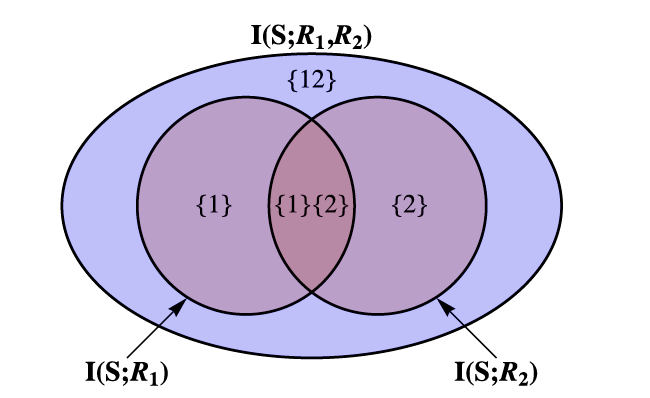
\includegraphics[height=5cm]{img/partial3.png}
%\caption{fig1}
\end{minipage}%
}%
\subfigure[4 Variables]{
\begin{minipage}[t]{0.5\linewidth}
\centering
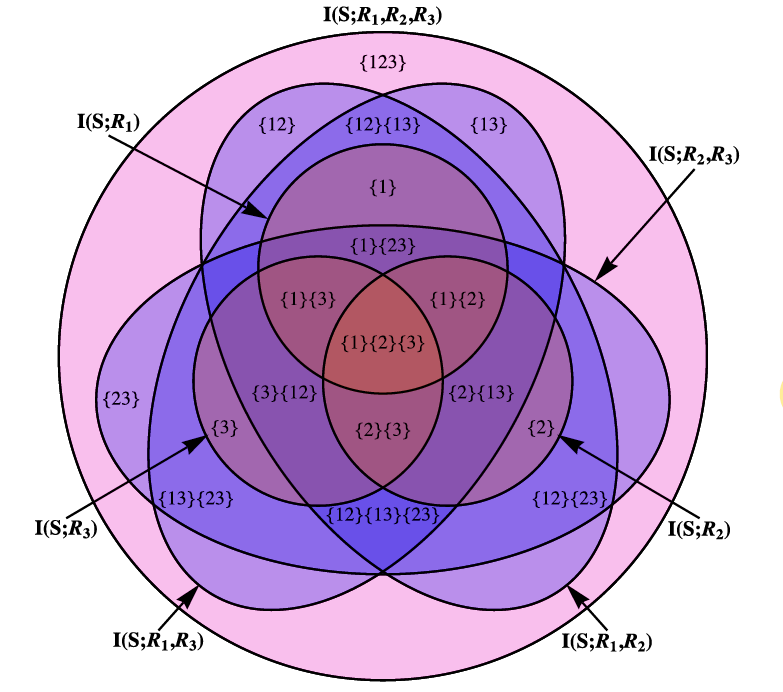
\includegraphics[height=5cm]{img/partial4.png}
%\caption{fig2}
\end{minipage}%
}%
\centering
\caption{Partial Information Diagrams}
\label{fig:pidiagram}
\end{figure}


Above all, we've formed a basic idea of the decomposition of partial information. We'll proceed to formulate how to measure these notions with set measure in the next chapter.




